\begin{titlepage}
%\AddToShipoutPicture*{\BackgroundIm}

   \begin{center}
       \vspace{-6cm}

       \huge{\textbf{\mytitle}}
       \vspace{0.2cm}

       \large{
    \begin{tikzpicture}
    \node[fill=white, fill opacity=1]{\textbf{\penname}}
    \end{tikzpicture}
    \vspace{0.2cm}

    \begin{tikzpicture}
    \node[fill=white, fill opacity=1]{\textbf{Supervisor:}}
    \end{tikzpicture}

    \begin{tikzpicture}
    \node[fill=white, fill opacity=1]{\textbf{Dr.~Dan Jones}}
    \end{tikzpicture}


    \begin{tikzpicture}
    \node[fill=white, fill opacity=1]{\textbf{British Antarctic Survey}}
    \end{tikzpicture}

    \vspace{0.5cm}

    \begin{tikzpicture}
    \node[fill=white,fill opacity=1]{\normalsize{\today}}
    \end{tikzpicture}
        }

\vspace{2.2cm}

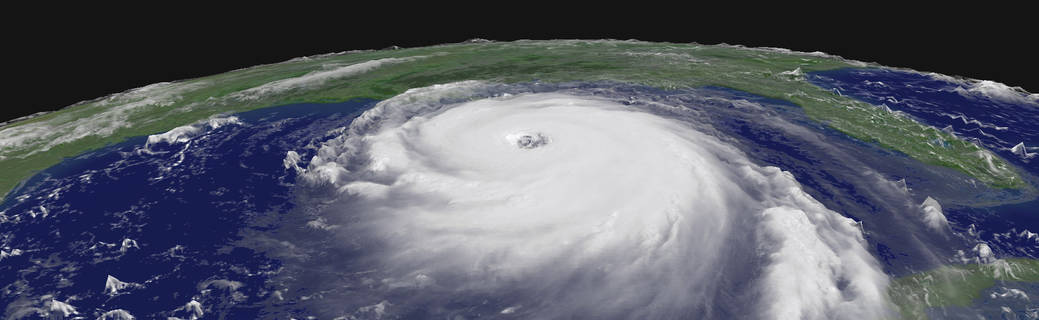
\includegraphics[width=\linewidth]{images/NASA-KATRINA-SIDEON.jpg}

   \vspace{2.2cm}
       \normalsize{
    \begin{tikzpicture}
    \node[fill=white,fill opacity=1]{A thesis submitted for the partial fulfilment of the
     }
    \end{tikzpicture}

    \begin{tikzpicture}
    \node[fill=white,fill opacity=1]{ degree requirements of Master of Natural Sciences.}
    \end{tikzpicture}
        }

       \vspace{0.4cm}


           \begin{tikzpicture}
    \node[fill=white,fill opacity=1] (a) {\large{
       \words~words}}
    \end{tikzpicture}
       \vspace{0.3cm}


       
\includegraphics[width=0.13\linewidth]{images/logos/UC.png}
       \vspace{0.8cm}
   \end{center}
\end{titlepage}

\newpage
    \addtocontents{toc}{\protect\thispagestyle{empty}}
  \vspace{-50pt}


  \tableofcontents

  \paragraph{Length compliance:}

  /limit \\
  Abstract:  \abwords/500 words. \\
  Main body: \words/5000 words, \pages/30 pages.\\

 \begin{table}[ht]
\resizebox{\columnwidth}{!}{%
\begin{tabular}{l L{7.5cm}}

\hline \hline
\textbf{Term} & \textbf{Definition}\\
\hline
Bathymetry & Depth of the ocean (relative to geoid)\\
Isobath & Bathymetry contour \\
Inundation & The flooding of the land \\
Barotropic & Fluid density is only a function of pressure\\
Baroclinic & Fluid density is \textbf{not} only a function of pressure \\
\hline \hline
\end{tabular}
}
\caption*{Table: Assumed oceanographic terms in this thesis,
that would not
be defined in a paper. }
\label{tab:oceanographic}
\end{table}

 Hazard is defined as,
 \begin{equation*}
 \mathrm{Hazard}\equiv \int_{\mathcal{S}} \int \mathrm{risk}(E, S)  \cdot \mathrm{harm}(E, S)\; dE\; dS,
 \end{equation*}
 where risk is the probability of an extreme event, level $E$,
 and harm is the amount of damage at that $E$, and $S$ is the position
 in the region $\mathcal{S}$.
  \thispagestyle{empty}

\newpage
